\documentclass[tikz,border=8pt]{standalone}
\usepackage{bm,amsmath}
\usetikzlibrary{arrows.meta, positioning, calc}

\begin{document}
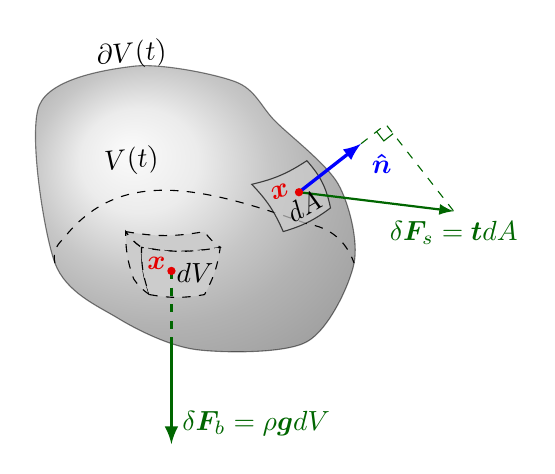
\begin{tikzpicture}
\usetikzlibrary{calc}
\shadedraw[ball color=gray!40,opacity=0.5] plot[smooth cycle] coordinates {(-2,1) (-0.8,1.5) (0.5,1.3) (1,0.8) (1.8,0) (2,-1) (1.4,-2) (0,-2.1) (-1,-1.7) (-1.8,-1)};
\draw[dashed] (-1.8,-1) to[bend left=30] (-1.7,-0.7) .. controls (-1,0.2) and (0,0) .. (1.4,-0.5) to [bend left=30] (2,-1);
\draw[fill=gray!40,opacity=0.7] (0.7,0) to[bend right=10] (1.4,0.3) to[bend left=15] (1.7,-0.3) to[bend left=10] (1.1,-0.6) to[bend right=10] cycle;
\node[rotate=5,anchor=south] at (-0.8,1.35) {$\partial V(t)$};
\node[rotate=5,anchor=south] at (-0.8,0) {$V(t)$};

\def\ang_n{38};
\coordinate (Px) at (1.3,-0.1);
\coordinate (Pn) at ($(Px)+(\ang_n:1)$);
\coordinate (Pf_n) at ($(Px)+(\ang_n:1.4)$);
\coordinate (Pf) at ($(Pf_n)+(\ang_n-90:1.4)$);
\draw[green!40!black,dashed] (Pn)-- (Pf_n)--(Pf) ;
\draw[green!40!black] ($(Pf_n)+(\ang_n:-0.15)$)--++(\ang_n-90:0.15)--++(\ang_n:0.15);
\draw[-latex,green!40!black,thick] (Px)--(Pf) node[pos=1,below] {$\delta\bm{F}_s=\bm{t}dA$};;
\draw[blue,very thick,-latex] (Px)--(Pn) node[below right] {$\bm{\hat{n}}$};
\node[anchor=center,rotate=30] at ($(Px)+(0.06,-0.18)$) {$dA$};
\fill[red!90!black] (Px) circle (1.5pt) node[above left=-0.1cm and -0.05cm,rotate=20] {$\bm{x}$};

%%% BODY FORCE
\coordinate (C1) at (-0.6,-1.4);
\coordinate (C2) at ($(C1)+(0.7,0)$);
\coordinate (C3) at ($(C2)+(0.2,0.6)$);
\coordinate (C4) at ($(C1)+(-0.1,0.6)$);
\coordinate (C5) at ($(C1)+(-0.2,0.2)$);
\coordinate (C6) at ($(C5)+(-0.1,0.6)$);
\coordinate (C7) at ($(C3)+(-0.2,0.2)$);

%\coordinate (G) at ($(C1)!0.4!(C2)$);
%\draw[very thick,dashed,green!40!black] (G)--++(0,-0.6);
%\draw[very thick,-latex,green!40!black] ($(G)+(0,-0.6)$)--++(0,-0.7) node[pos=1, below] {$\delta\bm{F}_b=\rho\bm{g}dV$}


\draw[fill=gray!40,dashed] (C1) to[bend left=10] (C5) to[bend left=10] (C6)
 to[bend right=10] (C4) to[bend right=10] cycle;

\draw[fill=gray!40,dashed] (C6) to[bend right=10] (C7) to[bend right=10] (C3) to[bend left=10] (C4) to[bend left=10] cycle;

\draw[fill=gray!40,dashed] (C1) to[bend right=10] (C2) to[bend right=10] (C3)
 to[bend left=10] (C4) to[bend right=10] cycle;

\coordinate (G) at ($(C1)!0.4!(C2)+(0,0.3)$);
\draw[very thick,dashed,green!40!black] (G)--++(0,-0.9);
\draw[very thick,-latex,green!40!black] ($(G)+(0,-0.9)$)--++(0,-1.3) node[pos=0.8, right] {$\delta\bm{F}_b=\rho\bm{g}dV$};



\node[anchor=south,yshift=-0.07cm,xshift=0.05cm] at ($(G)+(0.25,-0.2)$) {$dV$};
\fill[red!90!black] (G) circle (1.5pt) node[above left=-0.1cm and -0.05cm] {$\bm{x}$};


\end{tikzpicture}

\end{document}
